\chapter{Overview of the LHCb upgrade}
\label{ref:lhcb-upgrade-overview}

% General changes
The run 2 of LHC has reached its conclusion at the end of 2018.
It has entered the second long shutdown (LS2) period since then.
During this period,
the upgrade on the LHC has enabled the accelerator to operate at
an unprecedented center of mass energy $\sqrt{s} = 13.6$~TeV with an
instantaneous luminosity of $2 \times 10^{33}$~cm$^{-2}$~s$^{-1}$
(for LHCb, a five-fold increase compared to run 2's number.
CMS and ATLAS operate at a luminosity 10 times as large)
\cite{CERN_news:2022,Piucci_2017}.
As of now\footnote{
    As a reminder, ``now'' refers to November 2022.
}, some of the LHCb subdetectors, for example the Upstream Tracker, are still
being upgraded.

% Motivate the LHCb upgrade
The upgraded LHC, however, poses unique problems for the LHCb experiment:
%%%%
With current hardware triggers\footnote{
    As discussed in \cref{ref:detector:trigger},
    the hardware triggers require the event to be above a certain $\pt / E_T$
    threshold.
},
to maintain a constant readout rate of 1~MHz,
the thresholds for \pt and $E_T$ have to increase,
which largely cancels the benefit of running at higher luminosity.
As shown in \cref{fig:l0-trigger-eff},
the \pt-based hadronic trigger yields are saturating even at run 2 luminosity
($4 \times 10^{32}$~cm$^{-2}$~s$^{-1}$).
%%%%
In addition, at $2 \times 10^{33}$~cm$^{-2}$~s$^{-1}$ a significant portion of
bunch crossings contains $b$ and $c$ signals.
With the current inclusive trigger scheme,
there will be too many ``signal-like'' events to write offline on storage
\cite{Albrecht_2014}.

\begin{figure}[!htb]
    \centering
    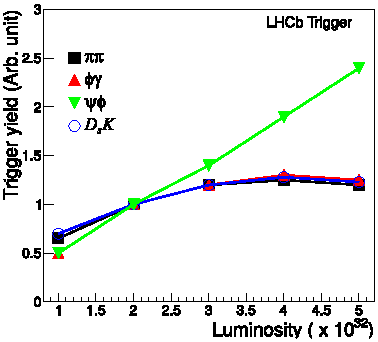
\includegraphics[width=0.5\textwidth]{./figs-lhcb-upgrade-overview/trigger_efficiency.pdf}
    \caption{
        L0 trigger yields normalized to that at
        $2 \times 10^{32}$~cm$^{-2}$s$^{-1}$.
        The hadronic triggers are already saturated at run 2 luminosity.
        Taken from \cite{CERN-LHCC-2011-001}.
    }
    \label{fig:l0-trigger-eff}
\end{figure}

To solve these problems, the detector readout rate is upgraded to 40~MHz,
the LHC bunch crossing rate,
without any hardware trigger.
By exposing all low-level variables to purely software-based high-level
triggers with more exclusive selection criteria,
events can be \emph{categorized} into exclusive signal decay modes more
efficiently with reasonable write throughputs.

Aside from the upgrade of the readout system and trigger scheme,
the tracking system is upgraded to provide better resolution and more
radiation tolerance to sustain the increased luminosity.
The subdetectors mainly used in L0 trigger, namely Muon station 1, SPD, and PS,
are removed altogether to reduce material in front of the calorimeters to
improve energy resolution.
The RICH1 detector which is responsible for PID is upgraded to reduce
occupancy\footnote{
    Defined as the fraction of detected photons over the total number of
    channels
    \cite{D_Ambrosio_2017}.
}
thus maintaining good PID efficiency.
The calorimeters (ECAL and HCAL) and the muon system will not undergo
substantial upgrades
\cite{Piucci_2017}.
The changes in the LHCb detector betwen run 1, 2 and run 3 are indicated
in \cref{fig:lhcb-detector-comparison}.

\begin{figure}[!htb]
    \centering
    \begin{subfigure}[t]{0.45\textwidth}
        \centering
        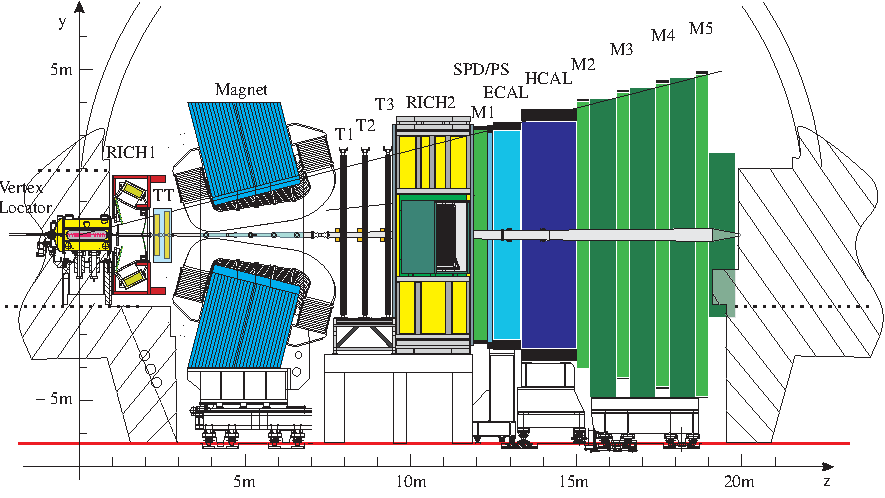
\includegraphics[width=\textwidth]{./figs-detector/lhcb_detector_view.pdf}
        \caption{The LHCb detector, run 1 and 2.}
    \end{subfigure}
    \hspace{12pt}
    %%%%
    \begin{subfigure}[t]{0.45\textwidth}
        \centering
        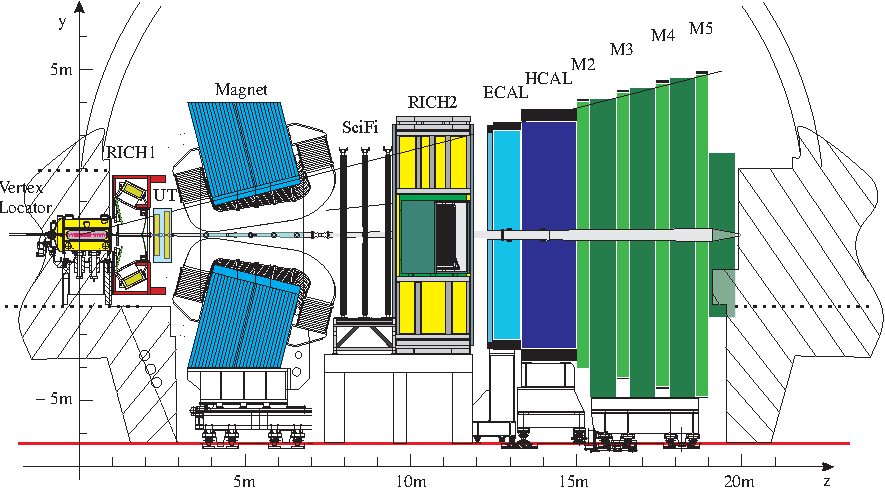
\includegraphics[width=\textwidth]{./figs-lhcb-upgrade-overview/lhcb_detector_view_run3.pdf}
        \caption{The upgraded LHCb detector in run 3.}
    \end{subfigure}

    \caption{
        The LHCb detector before (left) and after (right) LS2 upgrade.
        Note the upgrade on the tracking system:
        TT $\rightarrow$ UT, T-stations $\rightarrow$ SciFi;
        the removal of subdetectors relevant to L0 trigger only:
        The M1 muon station and SPD/PS have been removed.
    }
    \label{fig:lhcb-detector-comparison}
\end{figure}

The rest of the chapter provides an overview of the LHCb upgrade in LS2.
\cref{ref:lhcb-upgrade-overview:trigger}
provides an comparison of the trigger schemes between run 2 and run 3.
Some subdetectors are undergoing upgrade to improve its performance, notably
the tracking and the PID system;
these will be discussed in \cref{ref:lhcb-upgrade-overview:tracking} and
\cref{ref:lhcb-upgrade-overview:pid}, respectively.


\section{Trigger schemes in run 2 and run 3}
\label{ref:lhcb-upgrade-overview:trigger}

As can be seen in \cref{fig:trigger-comp},
the three main differences between run 2 and run 3 trigger scheme are:
The limited detector readout rate of 1~MHz is increased to 40~MHz\footnote{
    In the figure the frequency is labelled as ``30~MHz inelastic event rate''
    because it is the only type of collision that is visible to the LHCb
    detector.
    The readout rate is still 40~MHz, fully synchronous to the LHC frequency.
};
the storage write throughput is increased from 0.6~GB/s to 10~GB/s;
the HLT software triggers is capable of performing full event reconstruction at
the first stage, instead of partial reconstruction;
The implications of these differences are discussed in more details in the
following text.

\begin{figure}[!htb]
    \centering
    \begin{subfigure}[t]{0.36\textwidth}
        \centering
        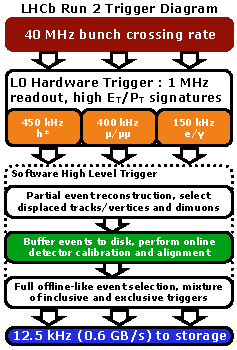
\includegraphics[width=\textwidth]{./figs-lhcb-upgrade-overview/trigger/trigger_scheme_run2.pdf}
        \caption{LHCb run 2 trigger scheme.}
    \end{subfigure}
    \hspace{20pt}
    %%%%
    \begin{subfigure}[t]{0.36\textwidth}
        \centering
        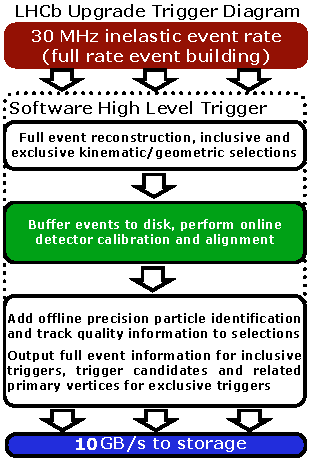
\includegraphics[width=\textwidth]{./figs-lhcb-upgrade-overview/trigger/trigger_scheme_run3.pdf}
        \caption{LHCb run 3 trigger scheme.}
    \end{subfigure}

    \caption{
        Comparison between run 2 and run 3 trigger schemes.
    }
    \label{fig:trigger-comp}
\end{figure}

The first point, reading out at 40~MHz, is due hadronic L0 trigger saturation,
which has been briefly discussed previously:
The hadronic L0 trigger requires the maximum energy $E_T$ deposited in the
calorimeters to be at least 3.7~GeV (for 2016) to reduce the triggering rate
at an acceptable level;
the threshold is already a significant portion of the $B$ meson mass
($\sim 5.3$~GeV).
Any further increase in luminosity requires an increase of the threshold,
which removes a significant portion of the signal events
that contain $B$ mesons,
resulting in an almost constant signal yield \cite{CERN-LHCC-2011-001}.

It begs the question then: Why don't we just make the detector readout at
40~MHz, while keeping the L0 triggers at current (or even lower) thresholds?
The second point, 10~GB/s write throughput,
comes into play.
This number is limited by the LAN connection speed from the LHCb on-site online
system (responsible for data acquisition) to CERN's storage center (Tier0) in
Meryin.
According to \cite{CERN-LHCC-2014-016},
there are 20 pairs of fibers, each is capable of transporting at 1~GB/s,
which, in theory, can provide a bandwidth of up to 20~GB/s.
Still, in the same reference, a maximum write throughput of 10~GB/s is
considered, perhaps due to concerns on robustness.
%%%%

At 13~TeV with a pile-up of 5.2 (similar to run 3 condition),
with a run 2-like inclusive trigger,
assuming an event size of 100~kB\footnote{
    The original text uses kb (kilo-bit), which does not add up to 80~GB/s for
    a 800~kHz rate.
    The size should be in kB (kilo-byte), as supported in
    \cite{CERN-LHCC-2014-016,Allen_GPU_2020}.
    The 800~kHz number is reported in \cite{LHCb-PUB-2014-027}.
},
the write throughput for beauty hadrons is 27~GB/s, for charm it is 80~GB/s,
for light long-lived particles (such as $K^0_S$ and $\Lambda^0$) 26~GB/s
\cite{Albrecht_2014},
far exceeding the bandwidth capacity.
In other words,
the old way of rejecting trivial backgrounds with minimal bias cuts on few
variables in an inclusive trigger is non-sustainable for LHCb run 3.
It is preferable to categorized different types of signals with as much
information from an event as possible, as early as possible
\cite{Albrecht_2014}.



\section{Tracking system}
\label{ref:lhcb-upgrade-overview:tracking}

% Get a figure for old IT/OT combo vs. the new SciFi


\section{Particle identification system}
\label{ref:lhcb-upgrade-overview:pid}


